%
% File: app0A.tex
% Author: Tengxiang Li
%
\chapter{Appendix A}
\begin{figure}[h]
    \centering
    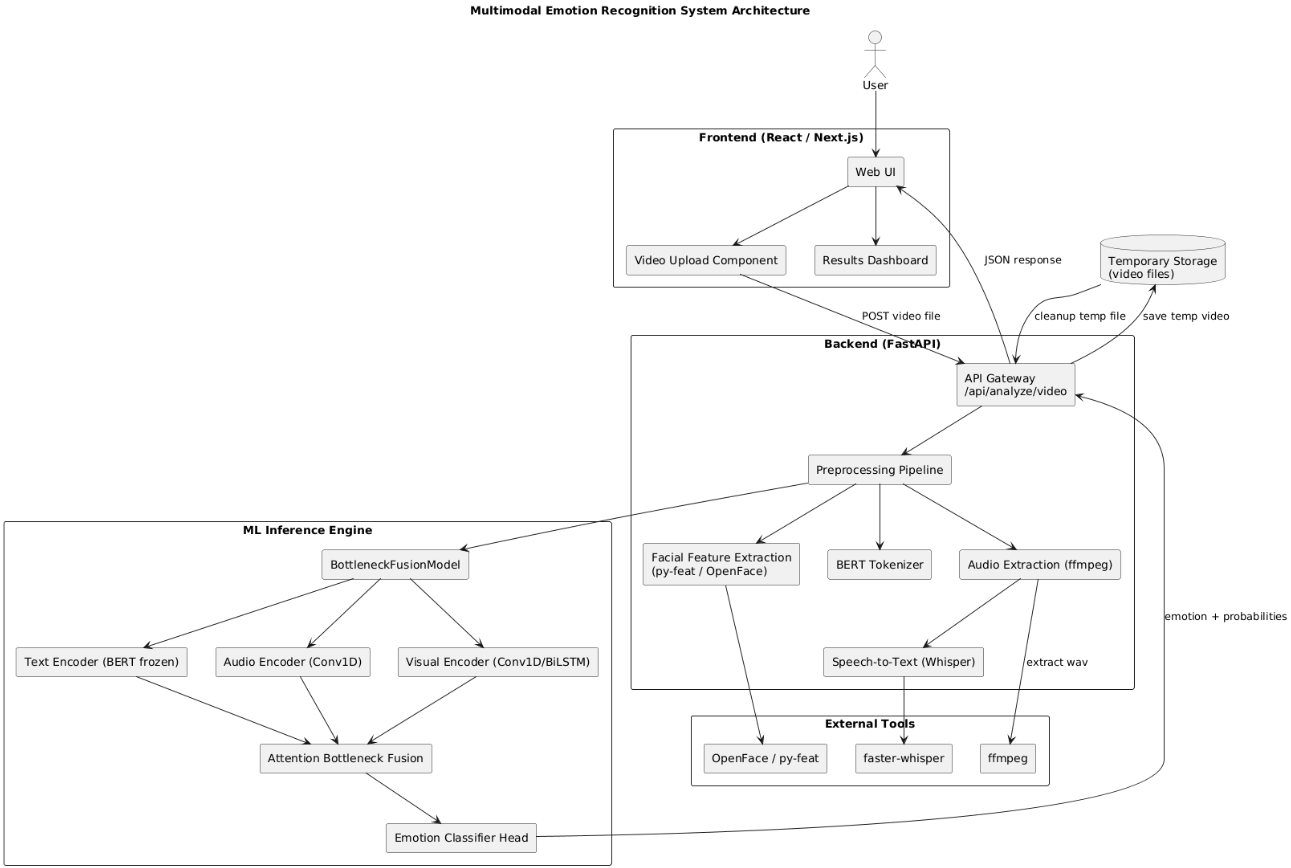
\includegraphics[width=1\textwidth]{images/image1.png}
    \caption{System Architecture}
    \label{fig:architecture}
\end{figure}




\chapter{Appendix B }

\begin{figure}[h]
    \centering
    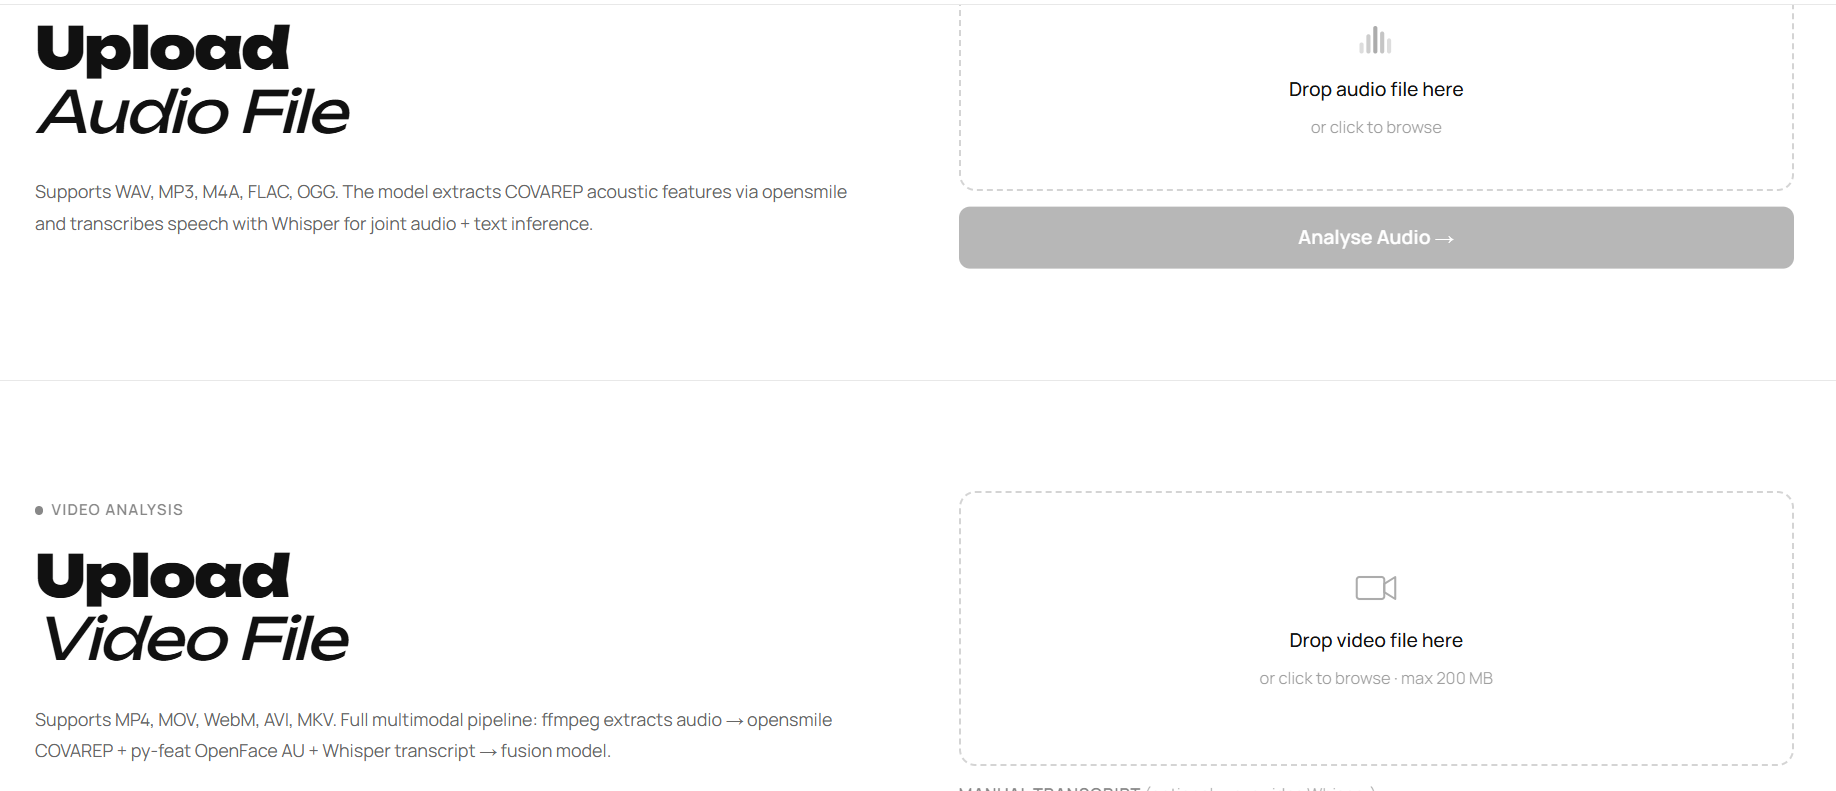
\includegraphics[width=1\textwidth]{images/image3.png}
    \label{fig:architecture}
\end{figure}

\begin{figure}[h]
    \centering
    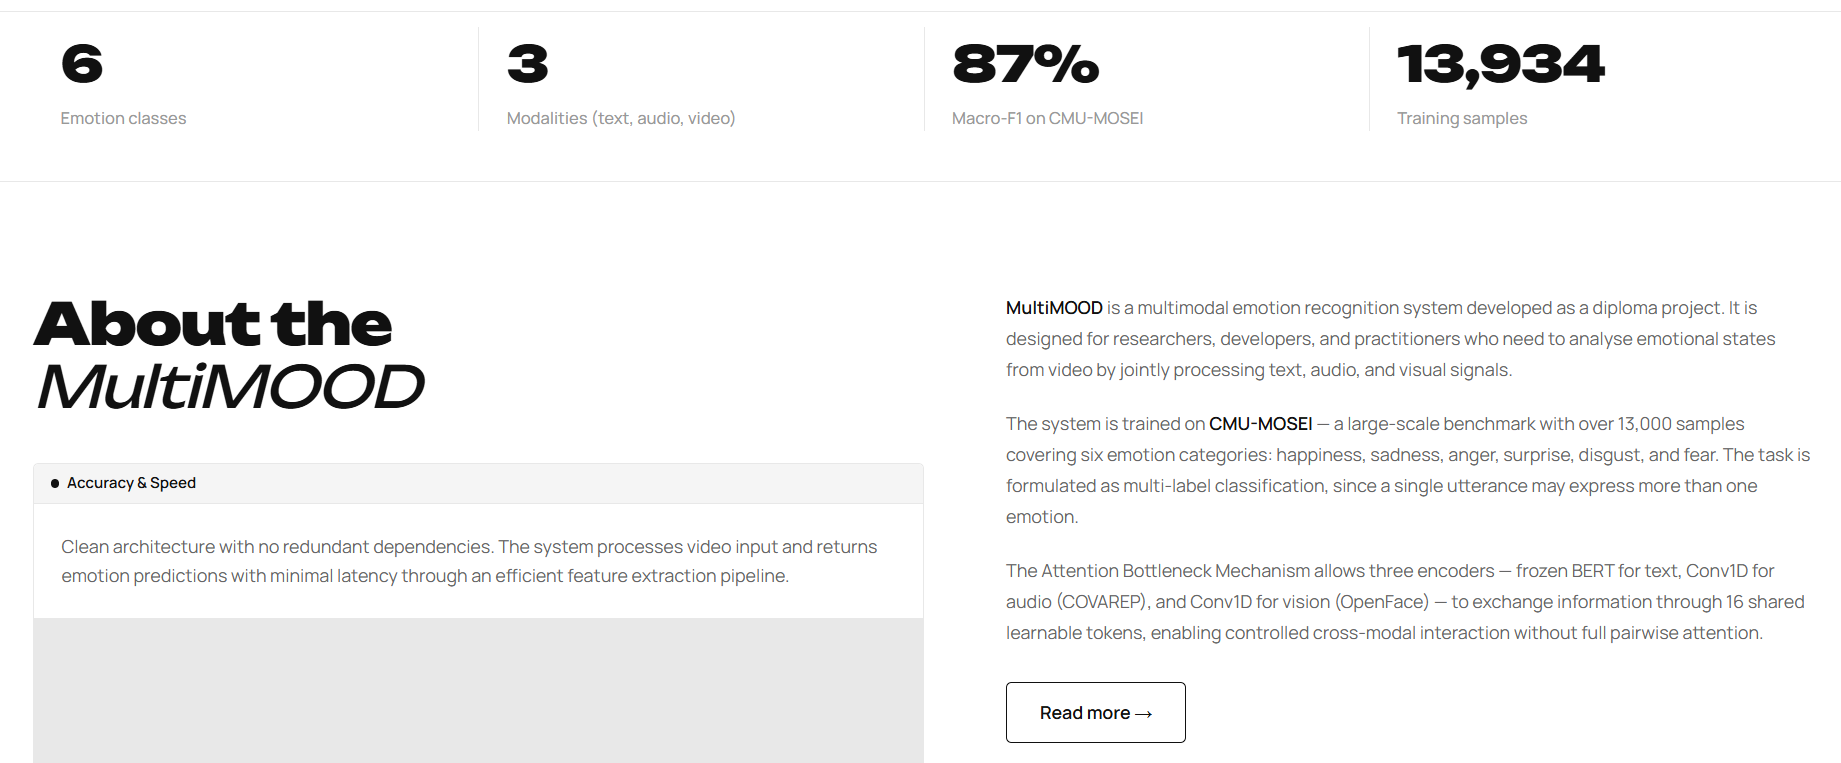
\includegraphics[width=1\textwidth]{images/image2.png}
    \caption{Frontend interface of the emotion recognition system}
    \label{fig:architecture}
\end{figure}

\begin{figure}[H]
    \centering
    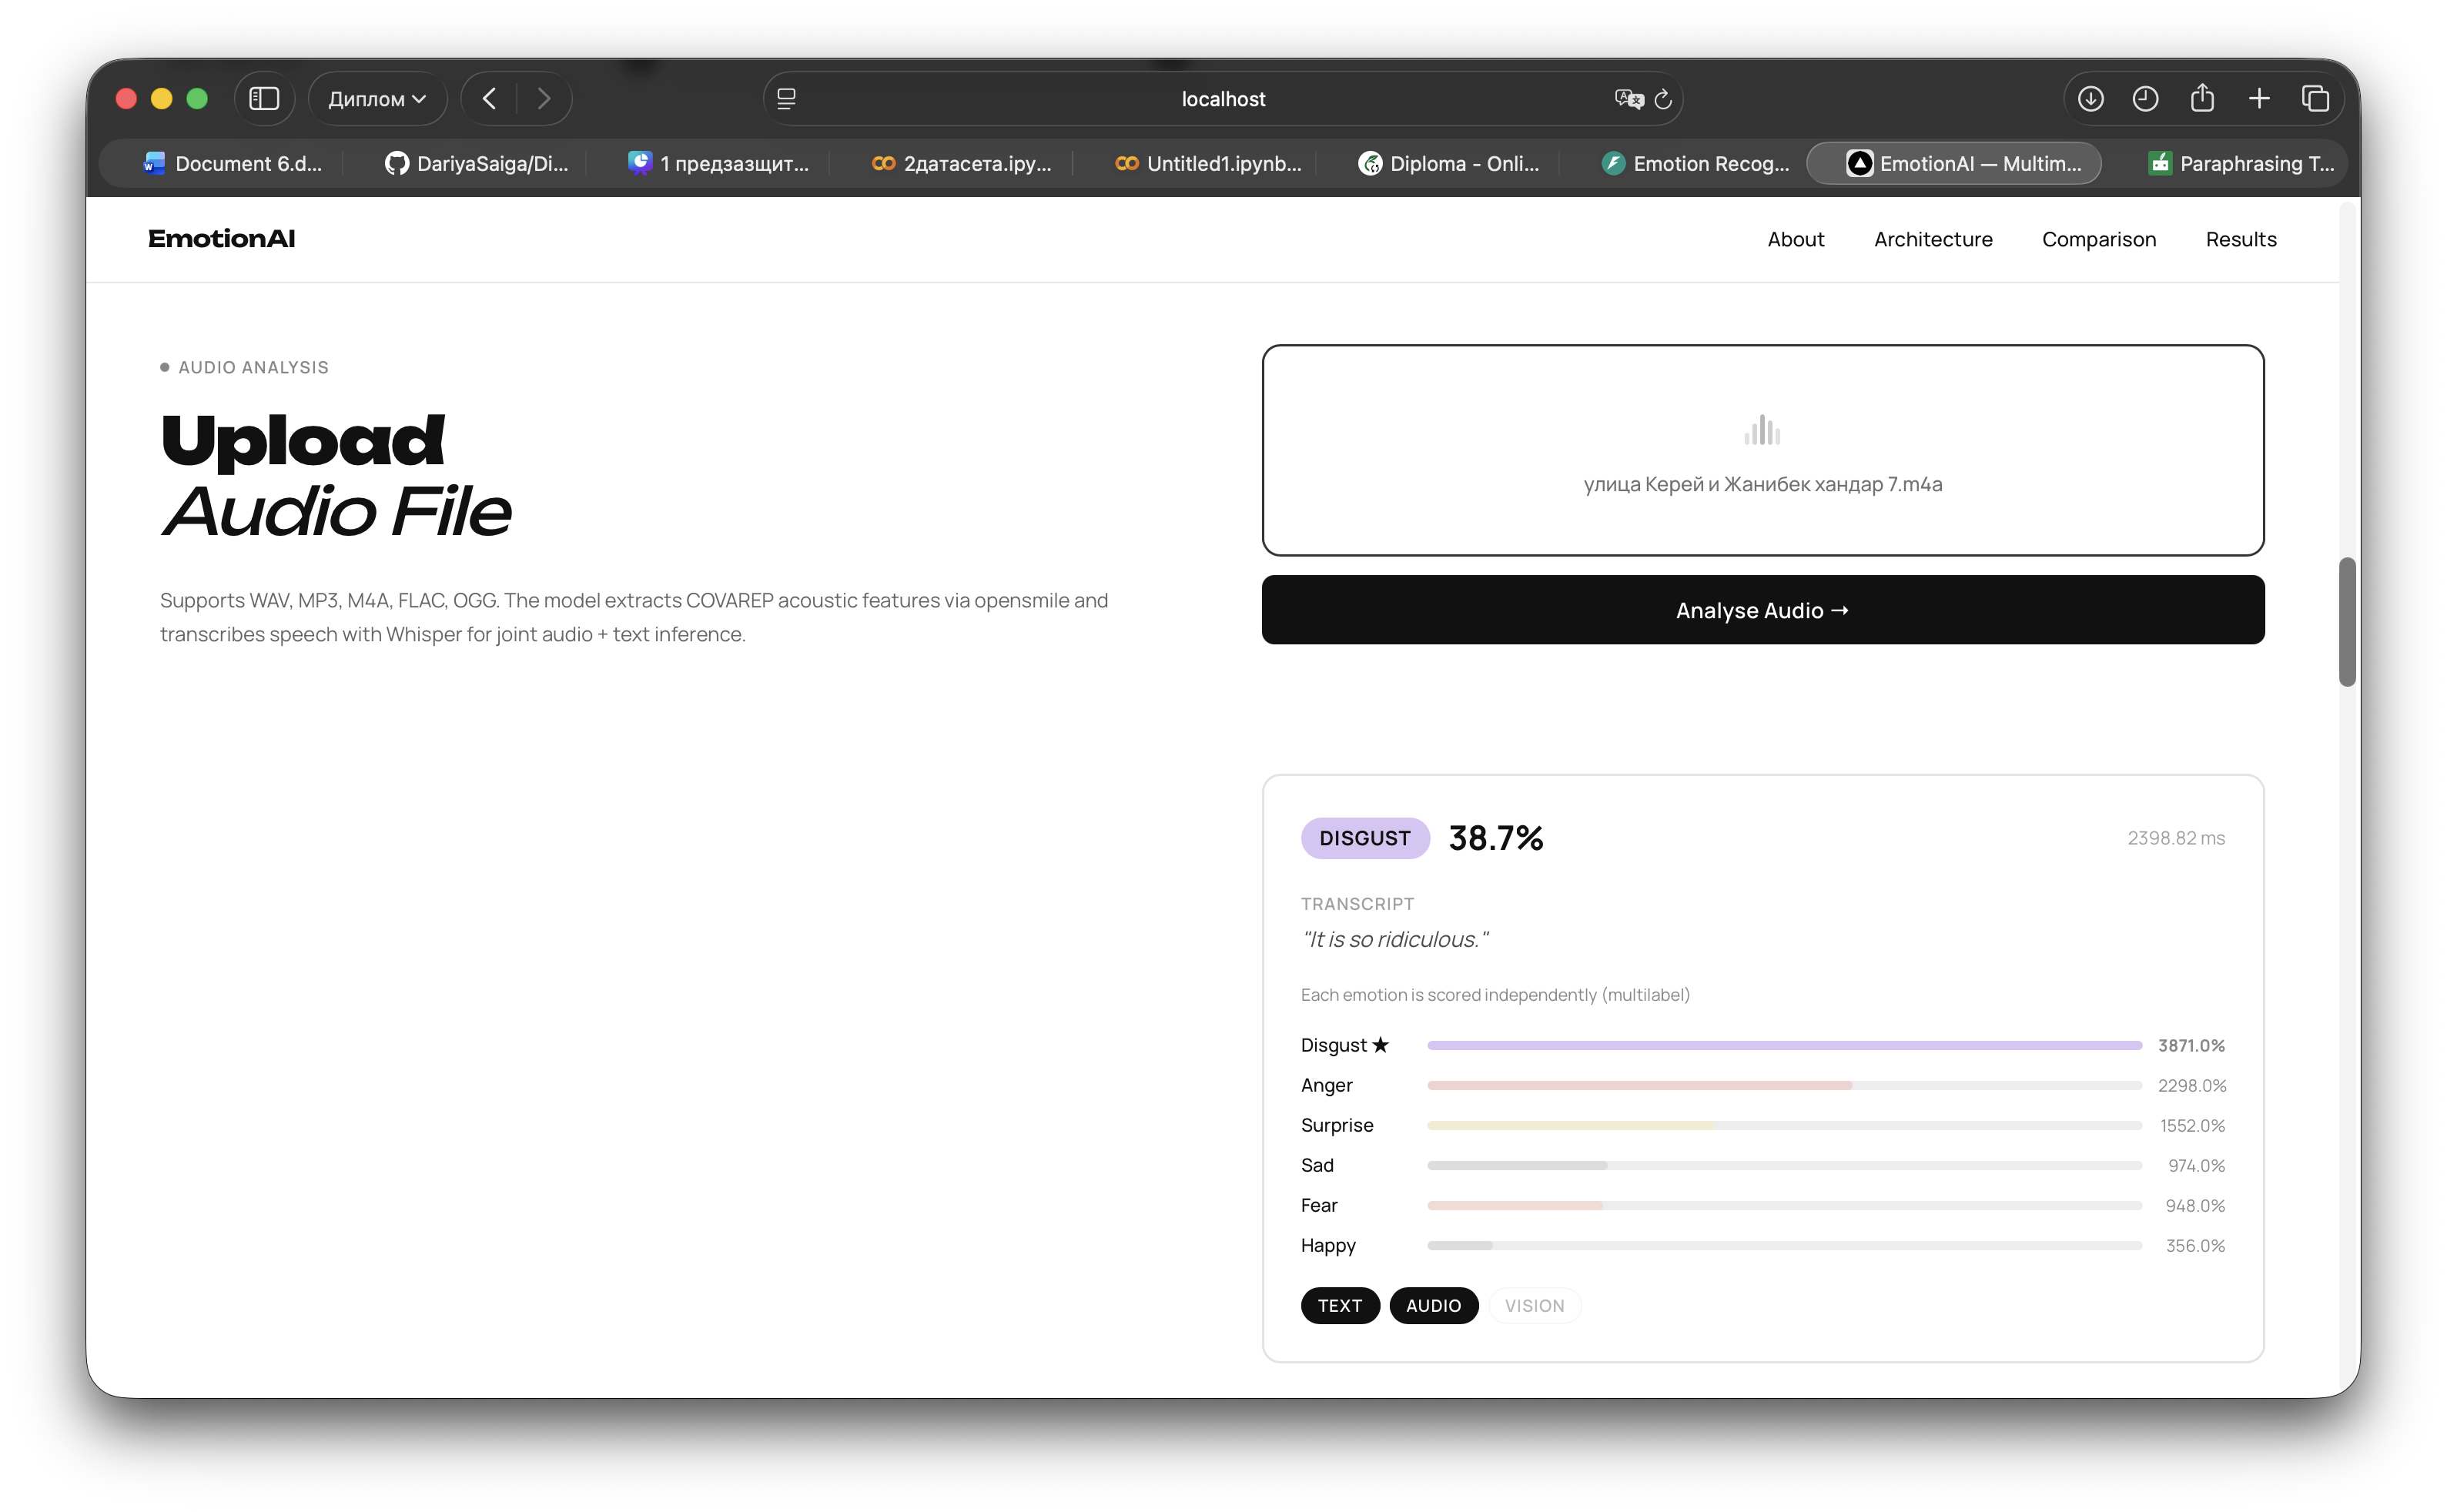
\includegraphics[width=1\textwidth]{images/audio_result.png}
    \caption{Audio modality prediction results}
    \label{fig:audio_result}
\end{figure}

\begin{figure}[H]
    \centering
    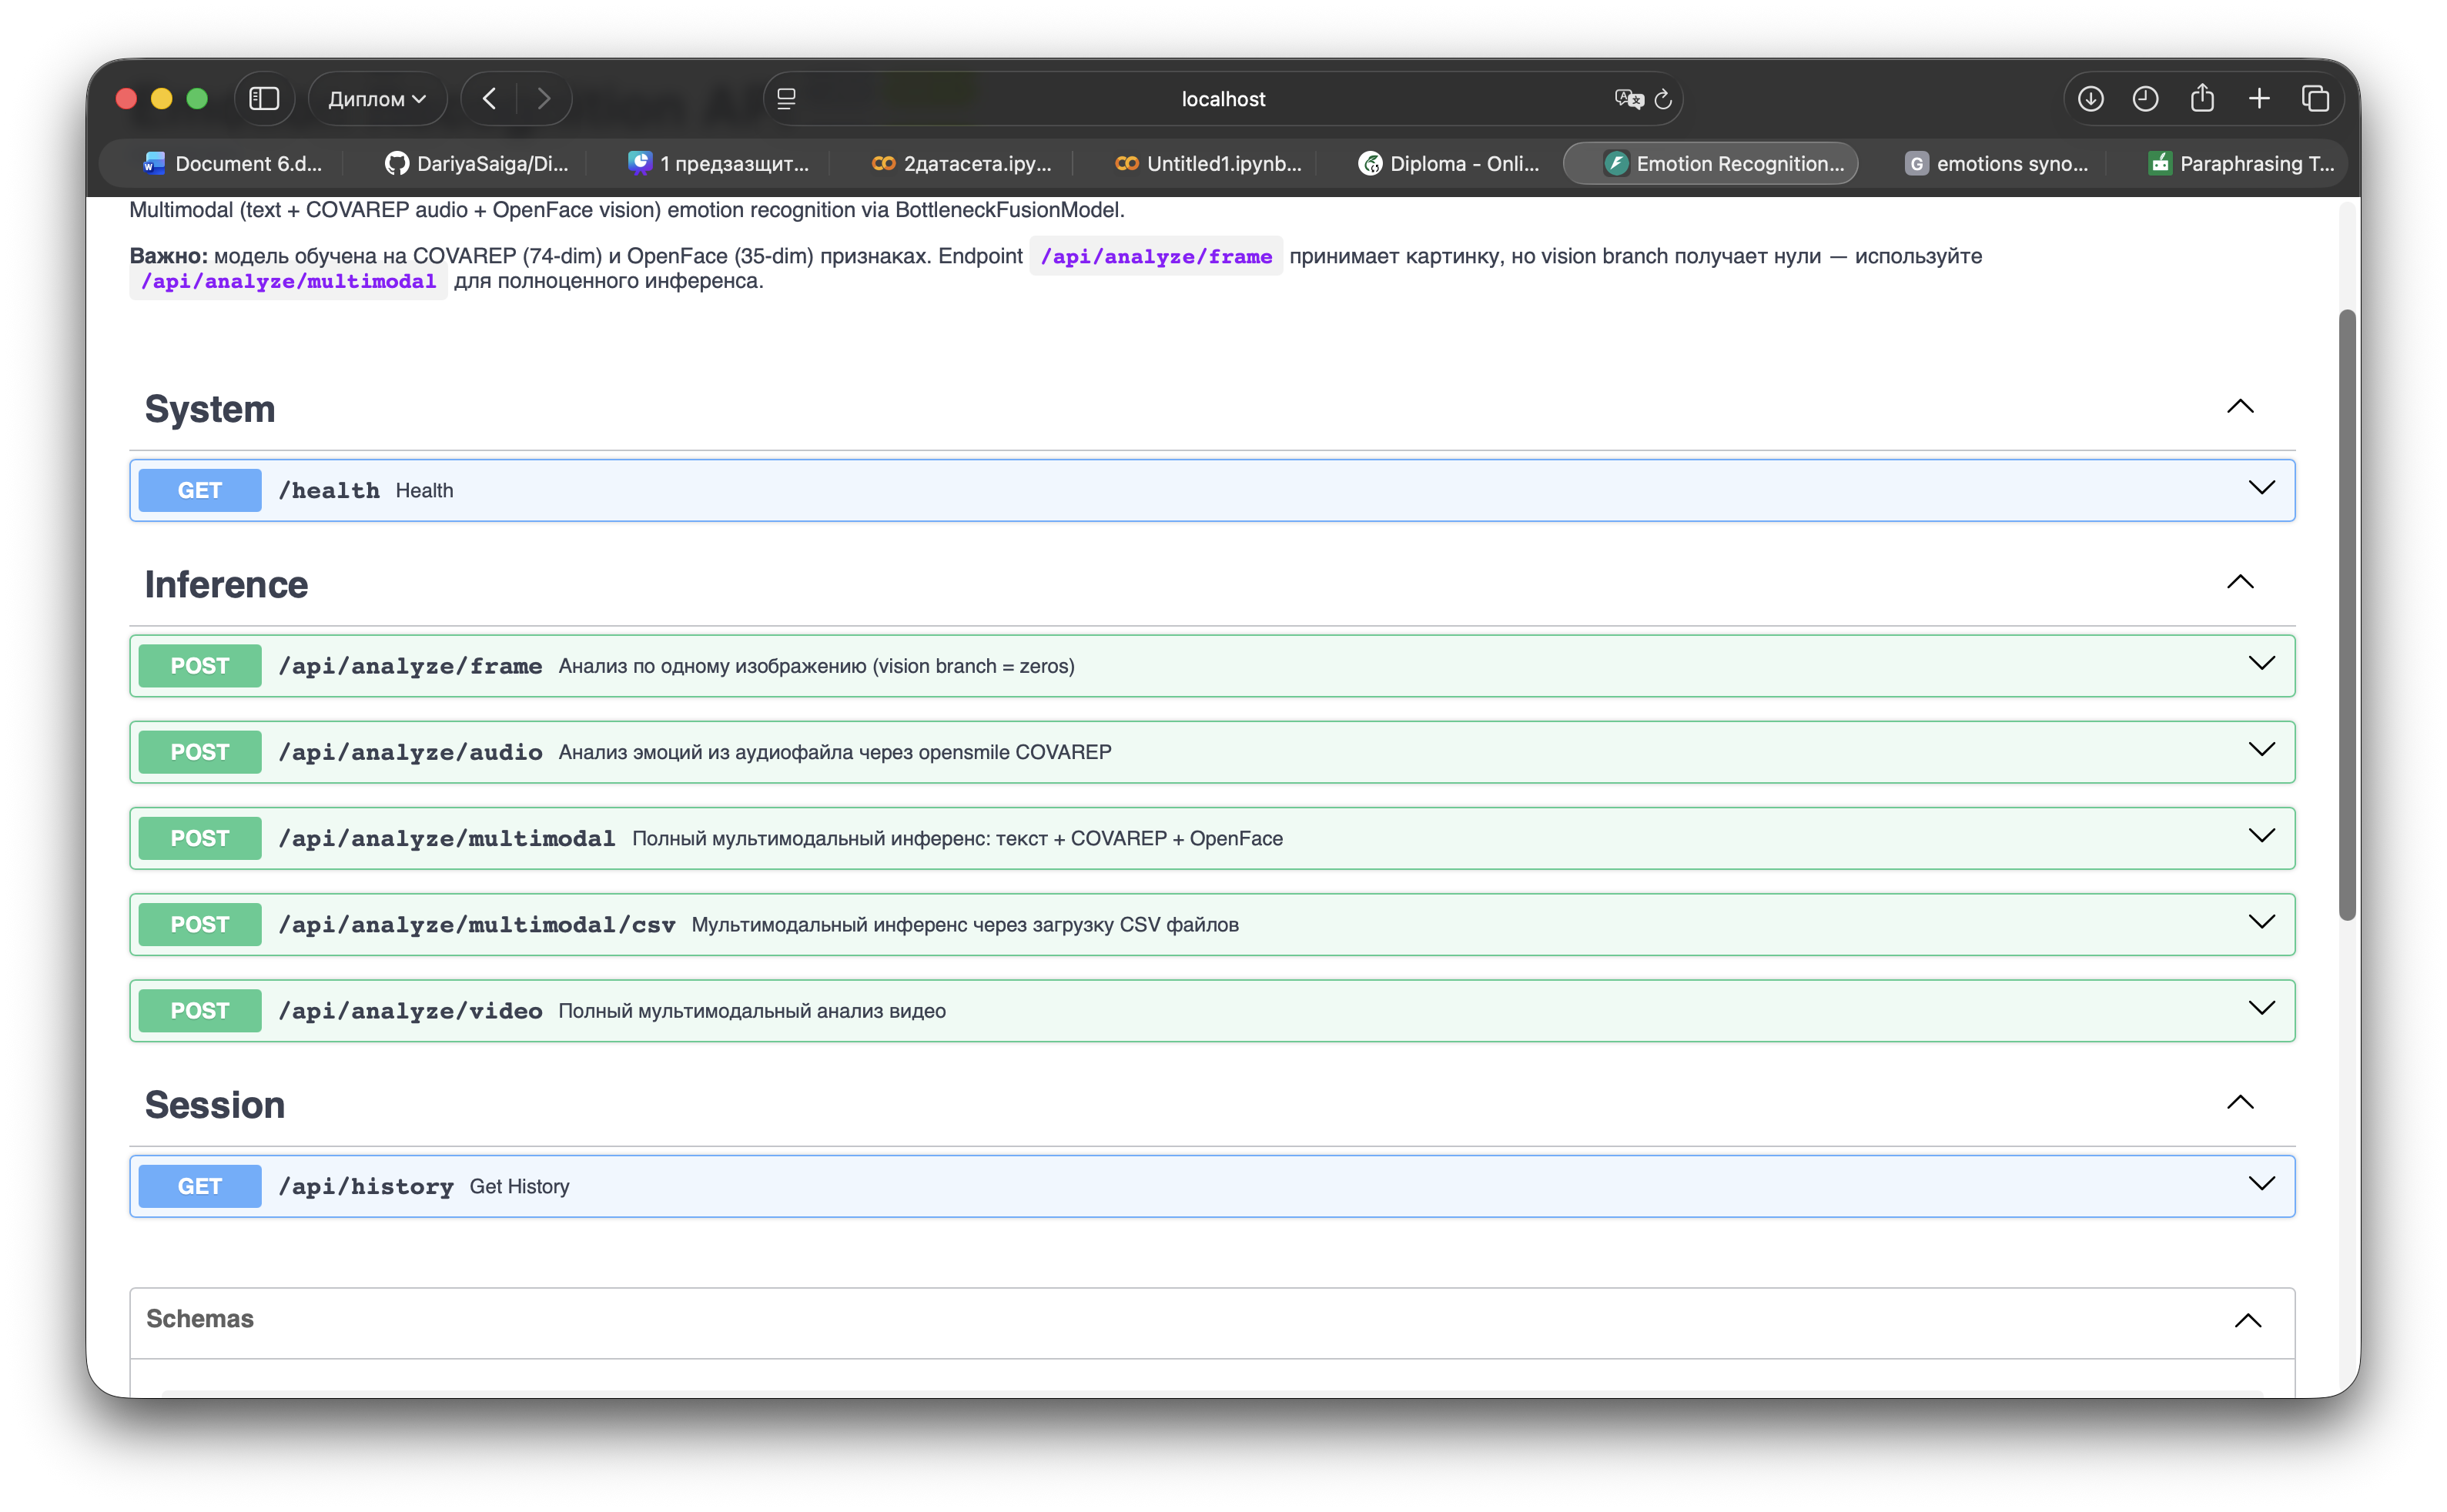
\includegraphics[width=1\textwidth]{images/backendpoint.png}
    \caption{Backend API endpoint configuration}
    \label{fig:backendpoint}
\end{figure}

\begin{figure}[H]
    \centering
    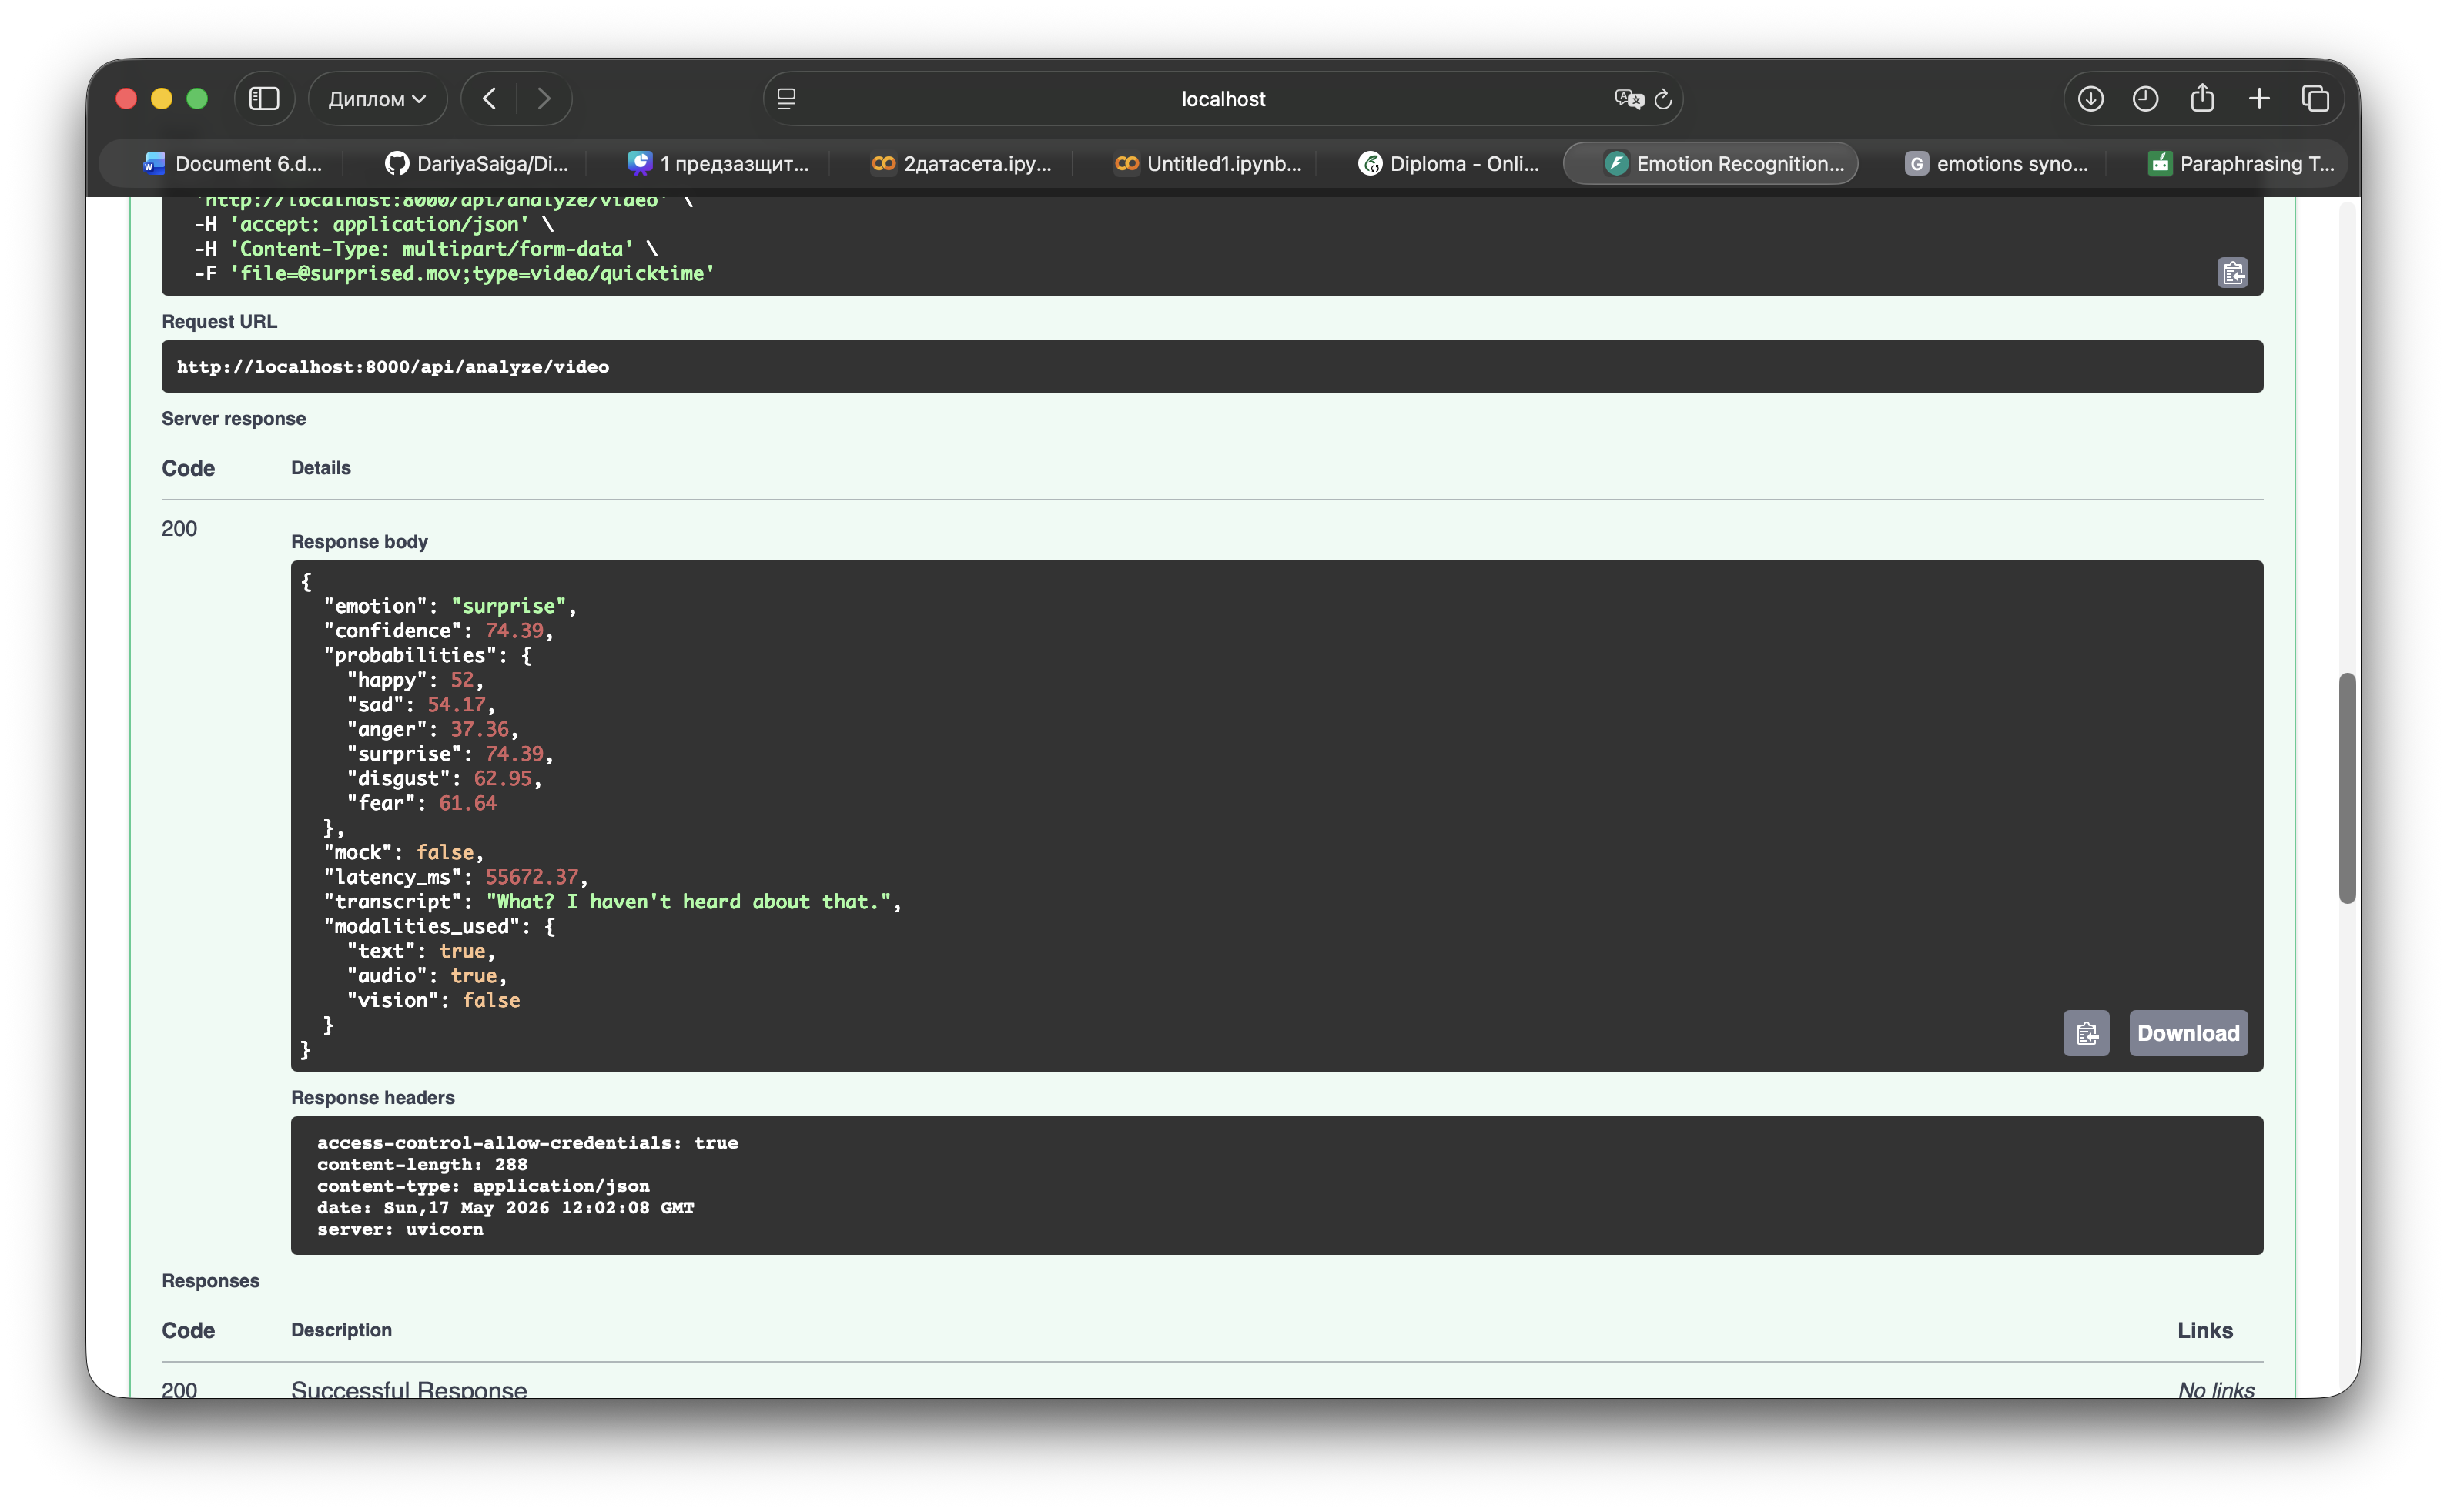
\includegraphics[width=1\textwidth]{images/back_result.png}
    \caption{Backend processing result output}
    \label{fig:back_result}
\end{figure}

\begin{figure}[H]
    \centering
    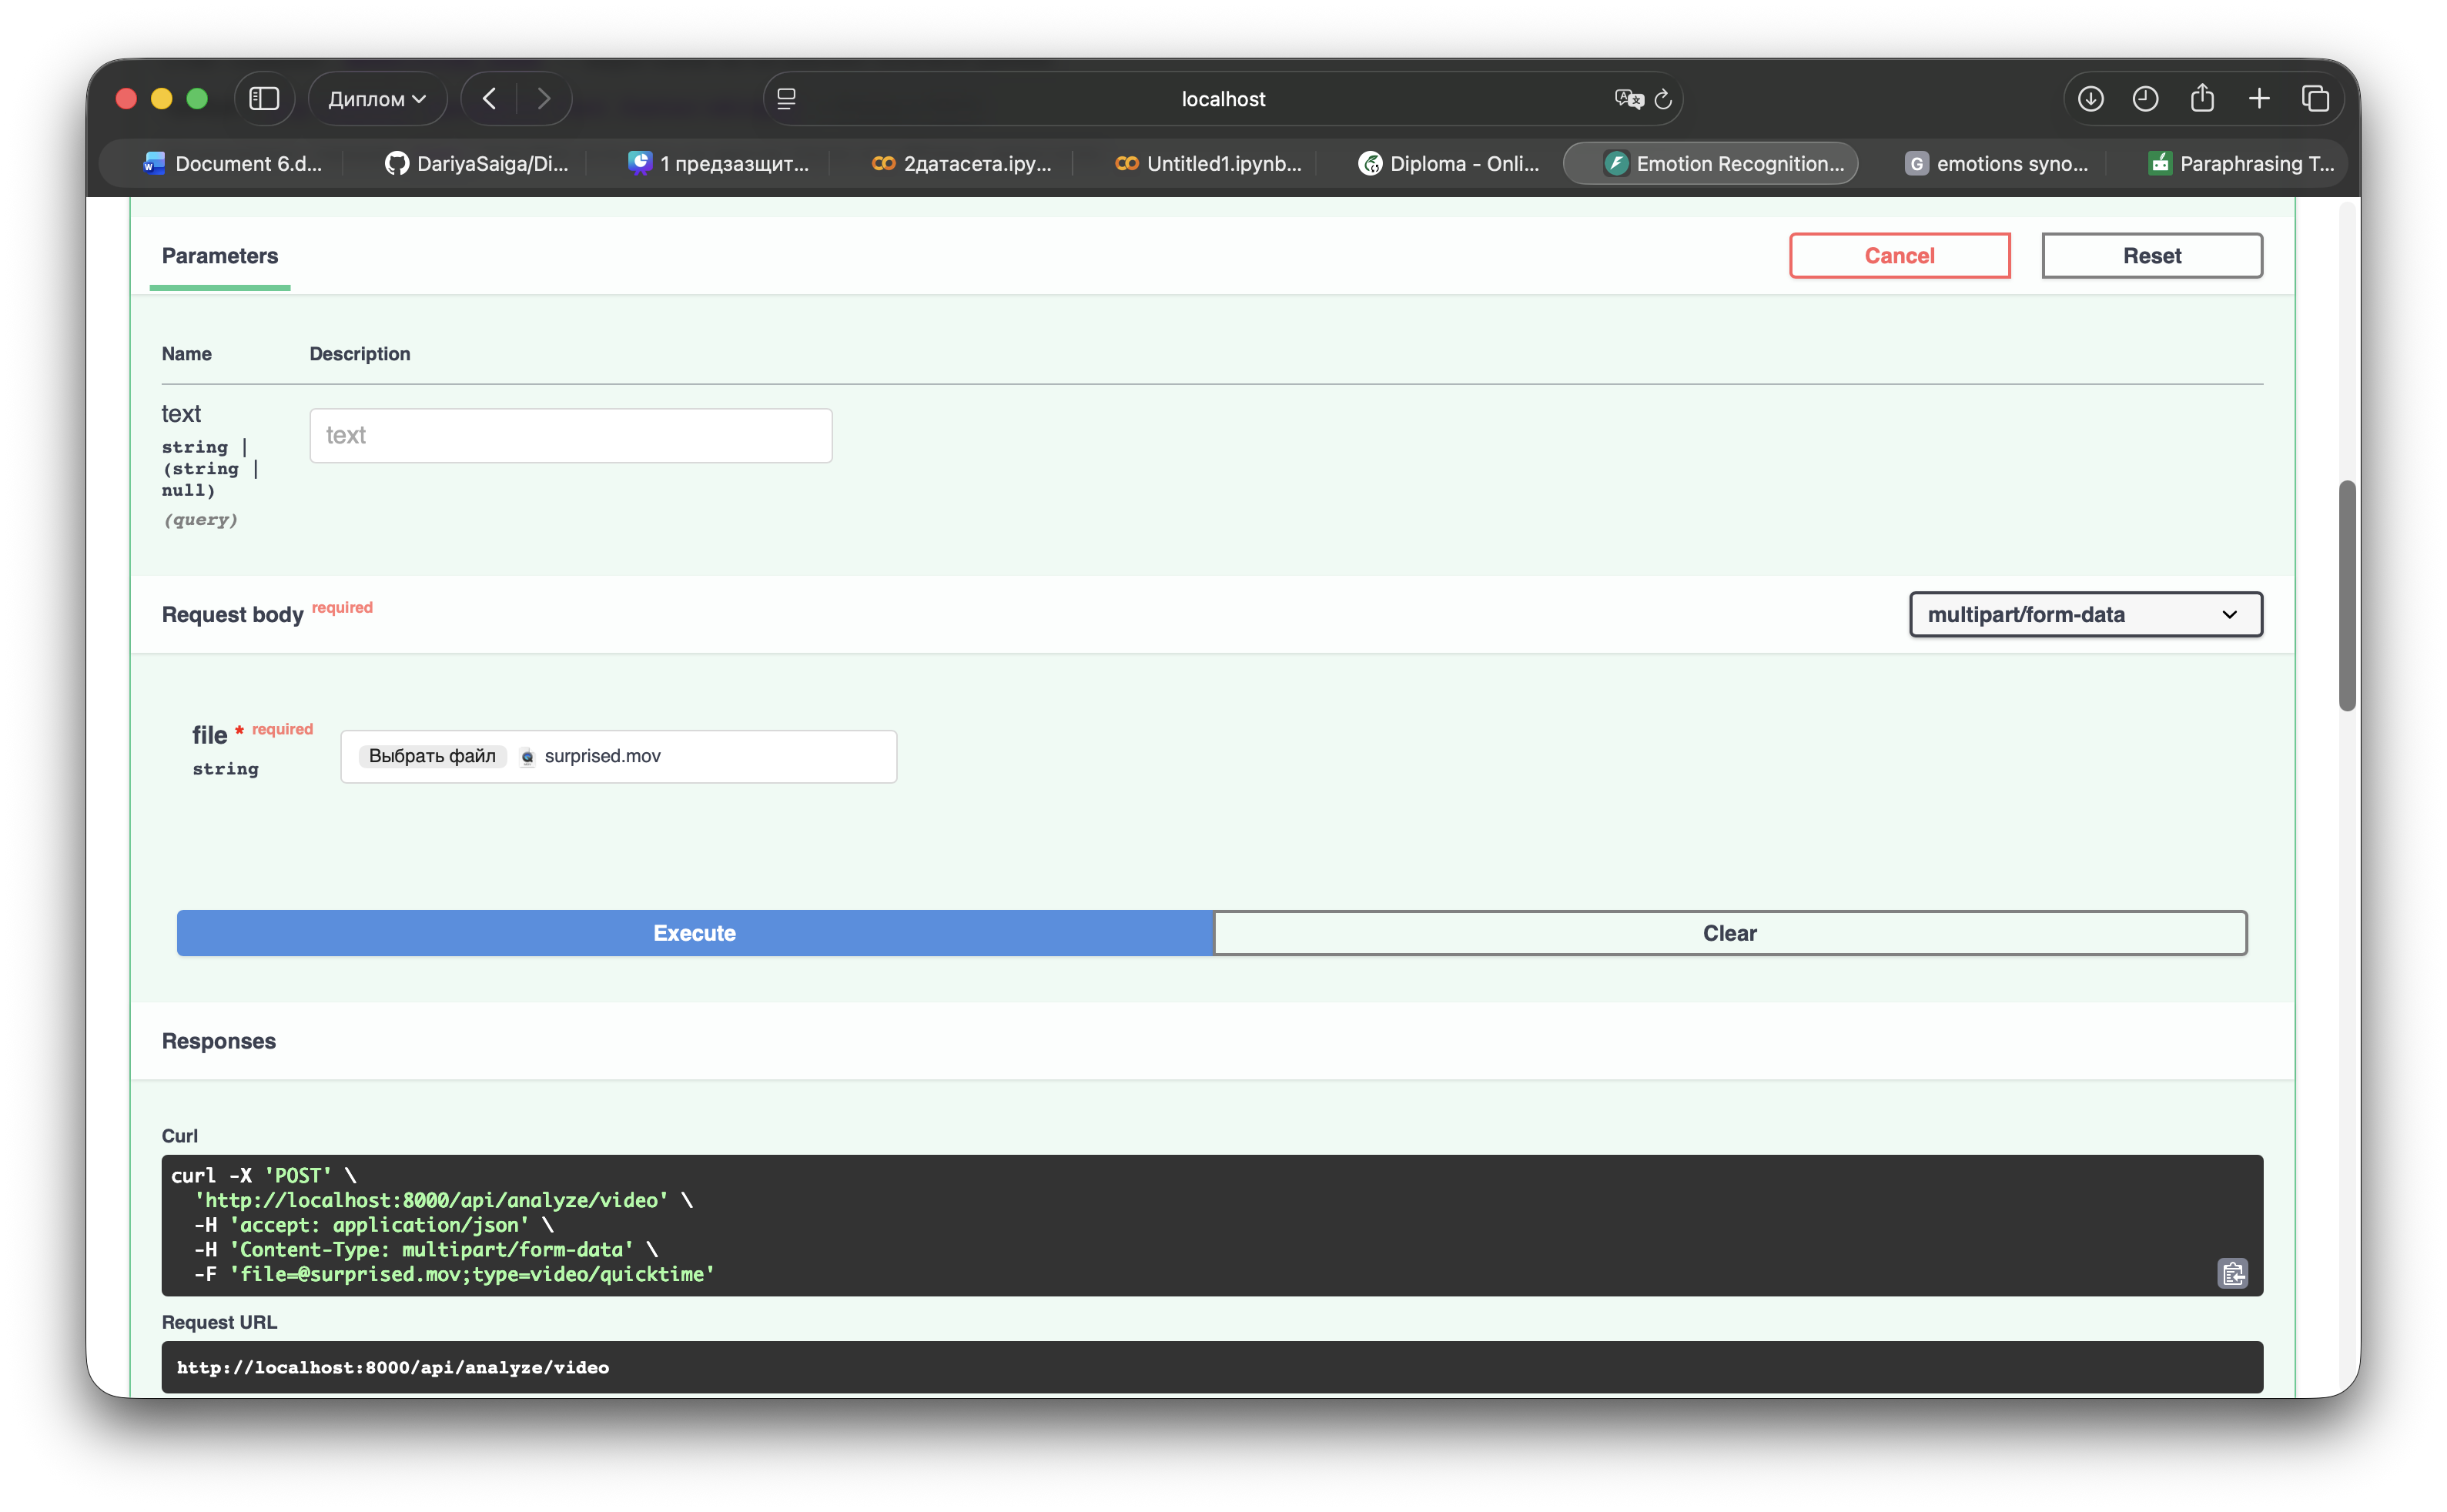
\includegraphics[width=1\textwidth]{images/back.png}
    \caption{Backend server interface}
    \label{fig:back}
\end{figure}


\chapter{Appendix C}
\begin{figure}[h]
    \centering
    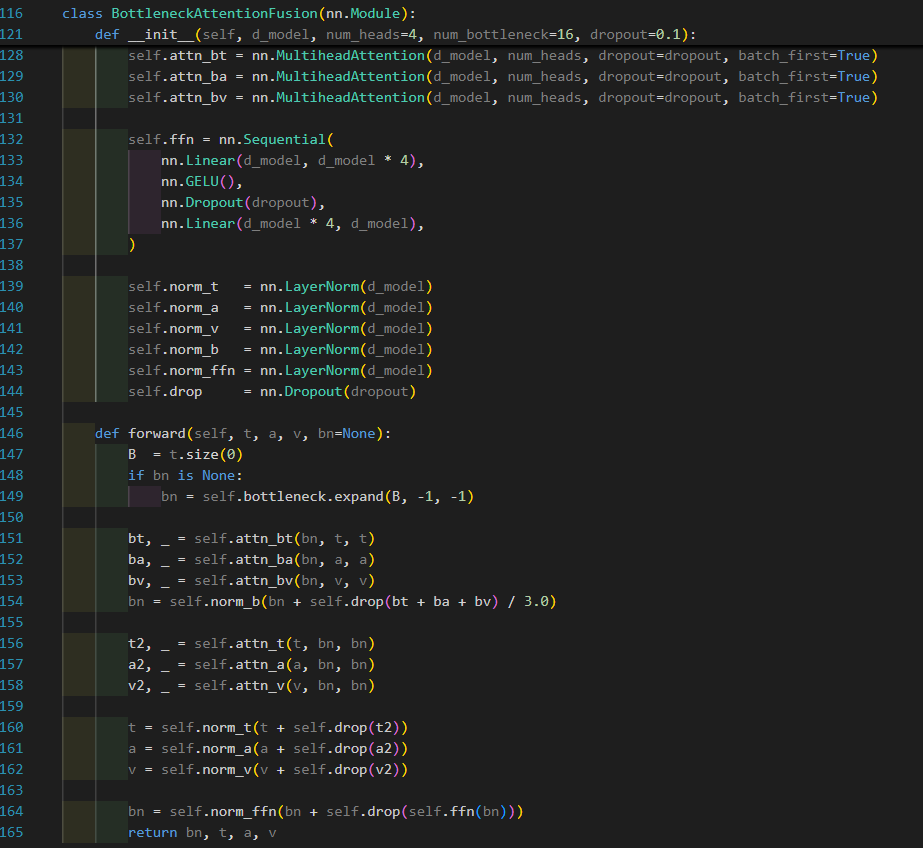
\includegraphics[width=1\textwidth]{images/image.png}
    \caption{Bottleneck Attention Fusion mechanism used in the multimodal model}
    \label{fig:architecture}
\end{figure}
\section{Bottleneck Attention Layer}
\begin{figure}[H]
    \centering
    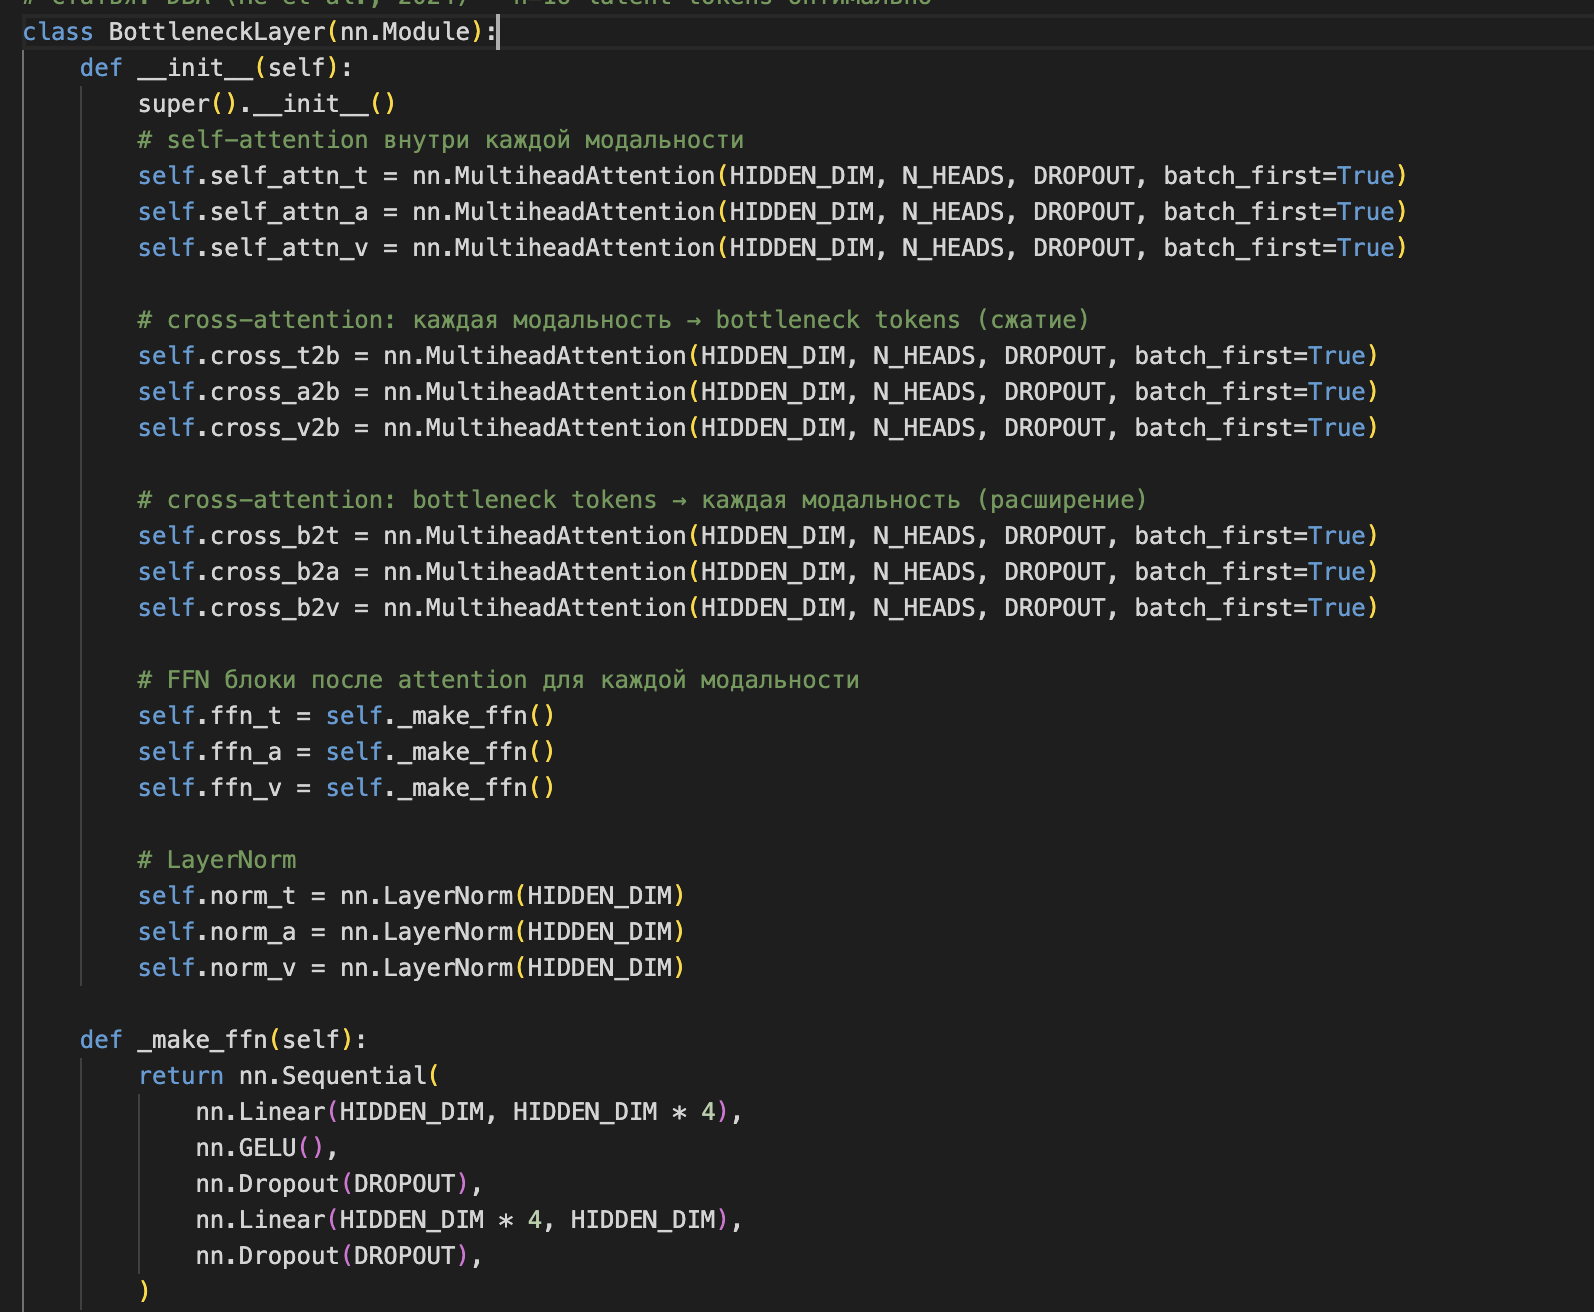
\includegraphics[width=1\textwidth]{images/bottleneckLayer.png}
    \caption{BottleneckLayer implementation in models.py}
    \label{fig:code_bottleneck}
\end{figure}

\section{Dataset Preprocessing}
\begin{figure}[H]
    \centering
    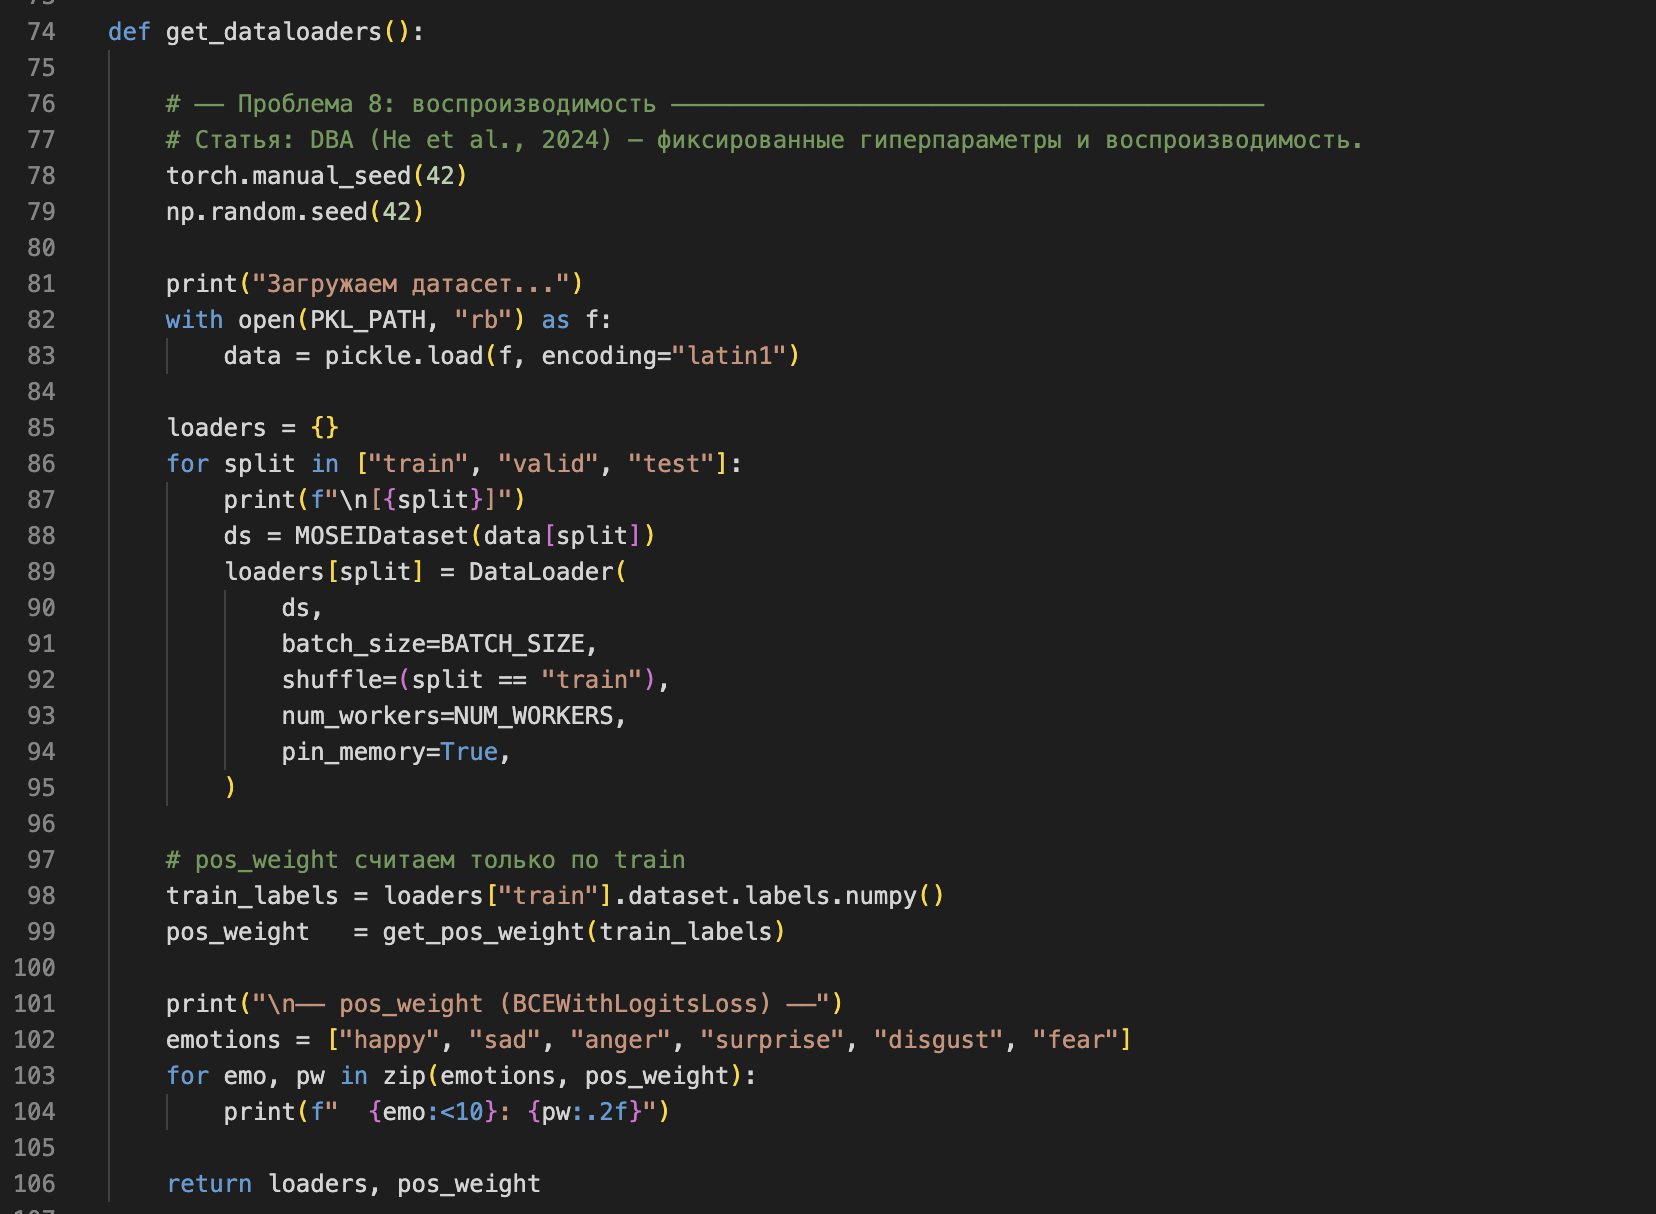
\includegraphics[width=1\textwidth]{images/dataset.png}
    \caption{Dataset loading and preprocessing pipeline}
    \label{fig:code_dataset}
\end{figure}

\section{Feature Extractor}
\begin{figure}[H]
    \centering
    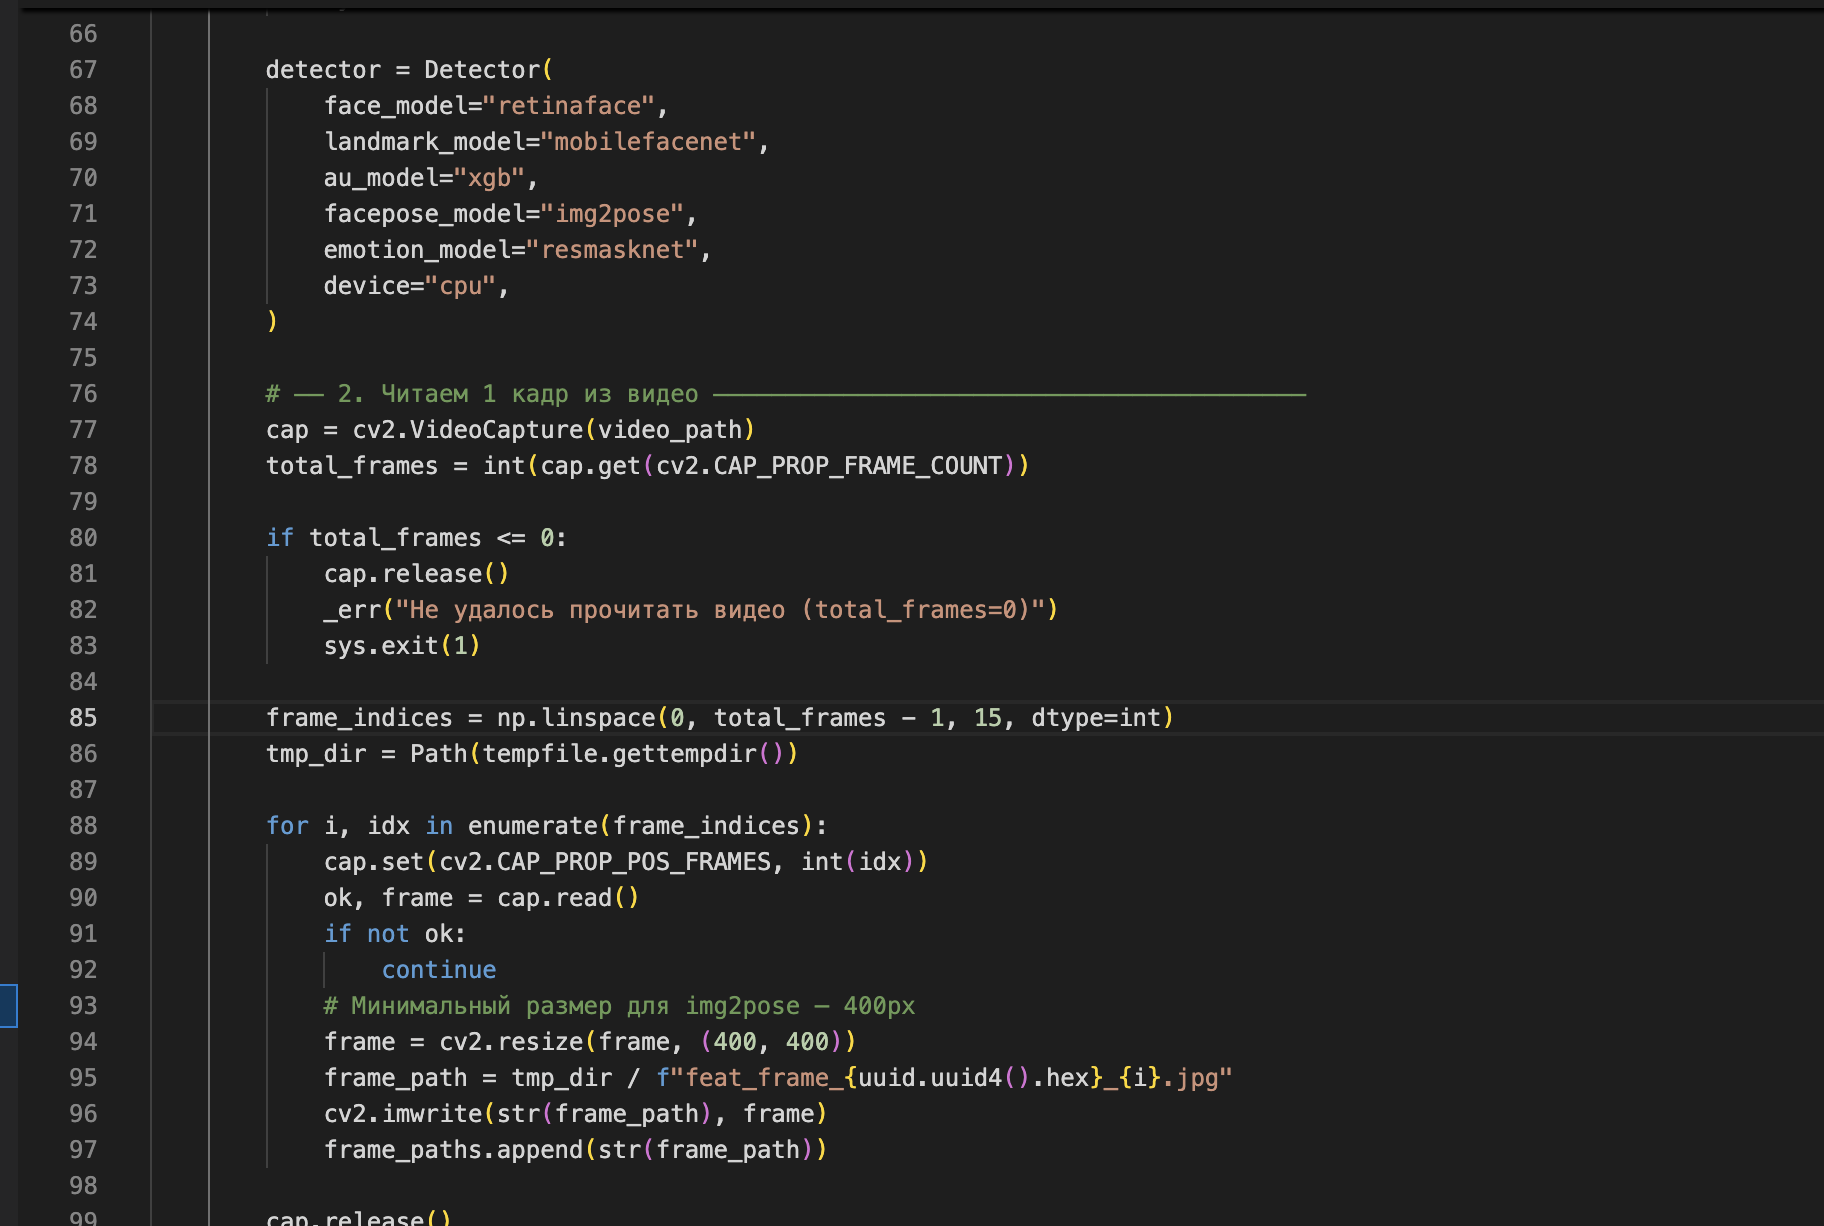
\includegraphics[width=1\textwidth]{images/detector.png}
    \caption{Visual feature extraction using py-feat}
    \label{fig:code_detector}
\end{figure}

\section{Training Loop}
\begin{figure}[H]
    \centering
    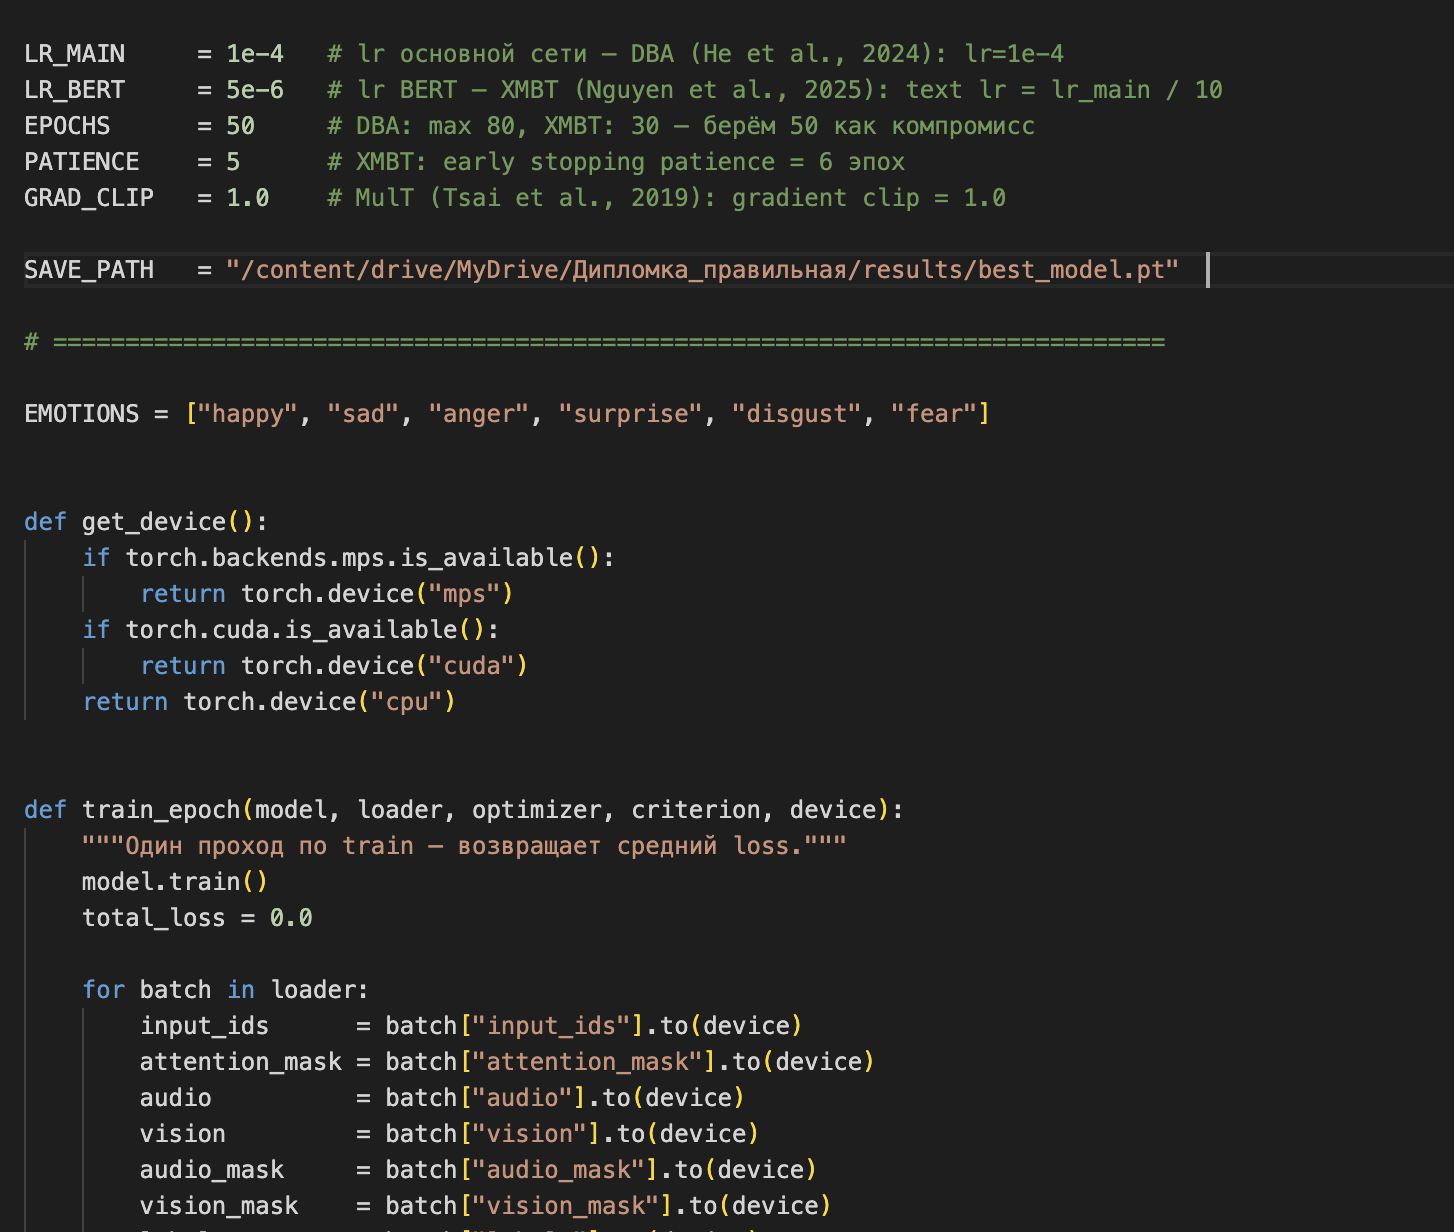
\includegraphics[width=1\textwidth]{images/train.png}
    \caption{Training loop implementation}
    \label{fig:code_train}
\end{figure}

\section{Train and Evaluate Functions}
\begin{figure}[H]
    \centering
    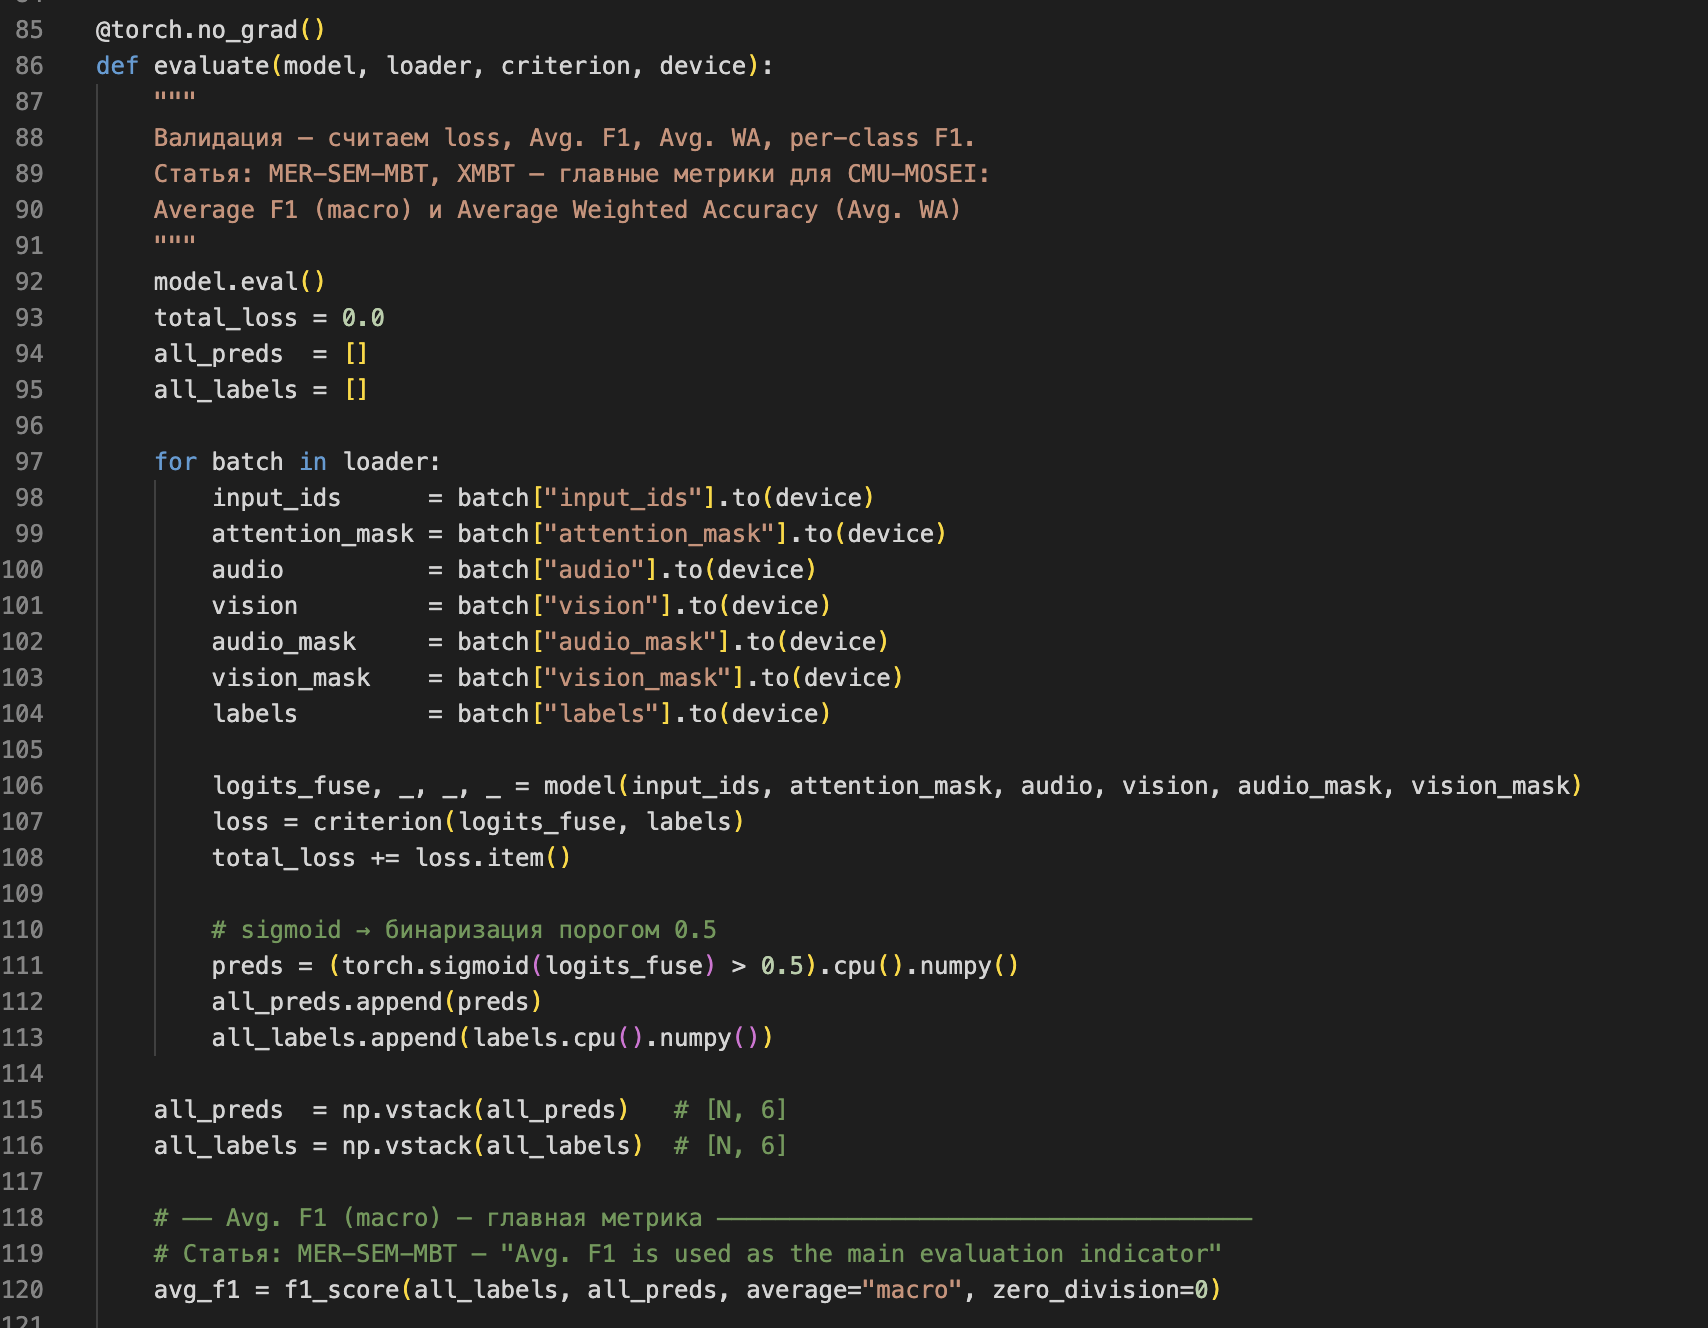
\includegraphics[width=1\textwidth]{images/trainevaluate.png}
    \caption{train\_epoch and evaluate functions}
    \label{fig:code_evaluate}
\end{figure}

\section{Video Feature Extraction}
\begin{figure}[H]
    \centering
    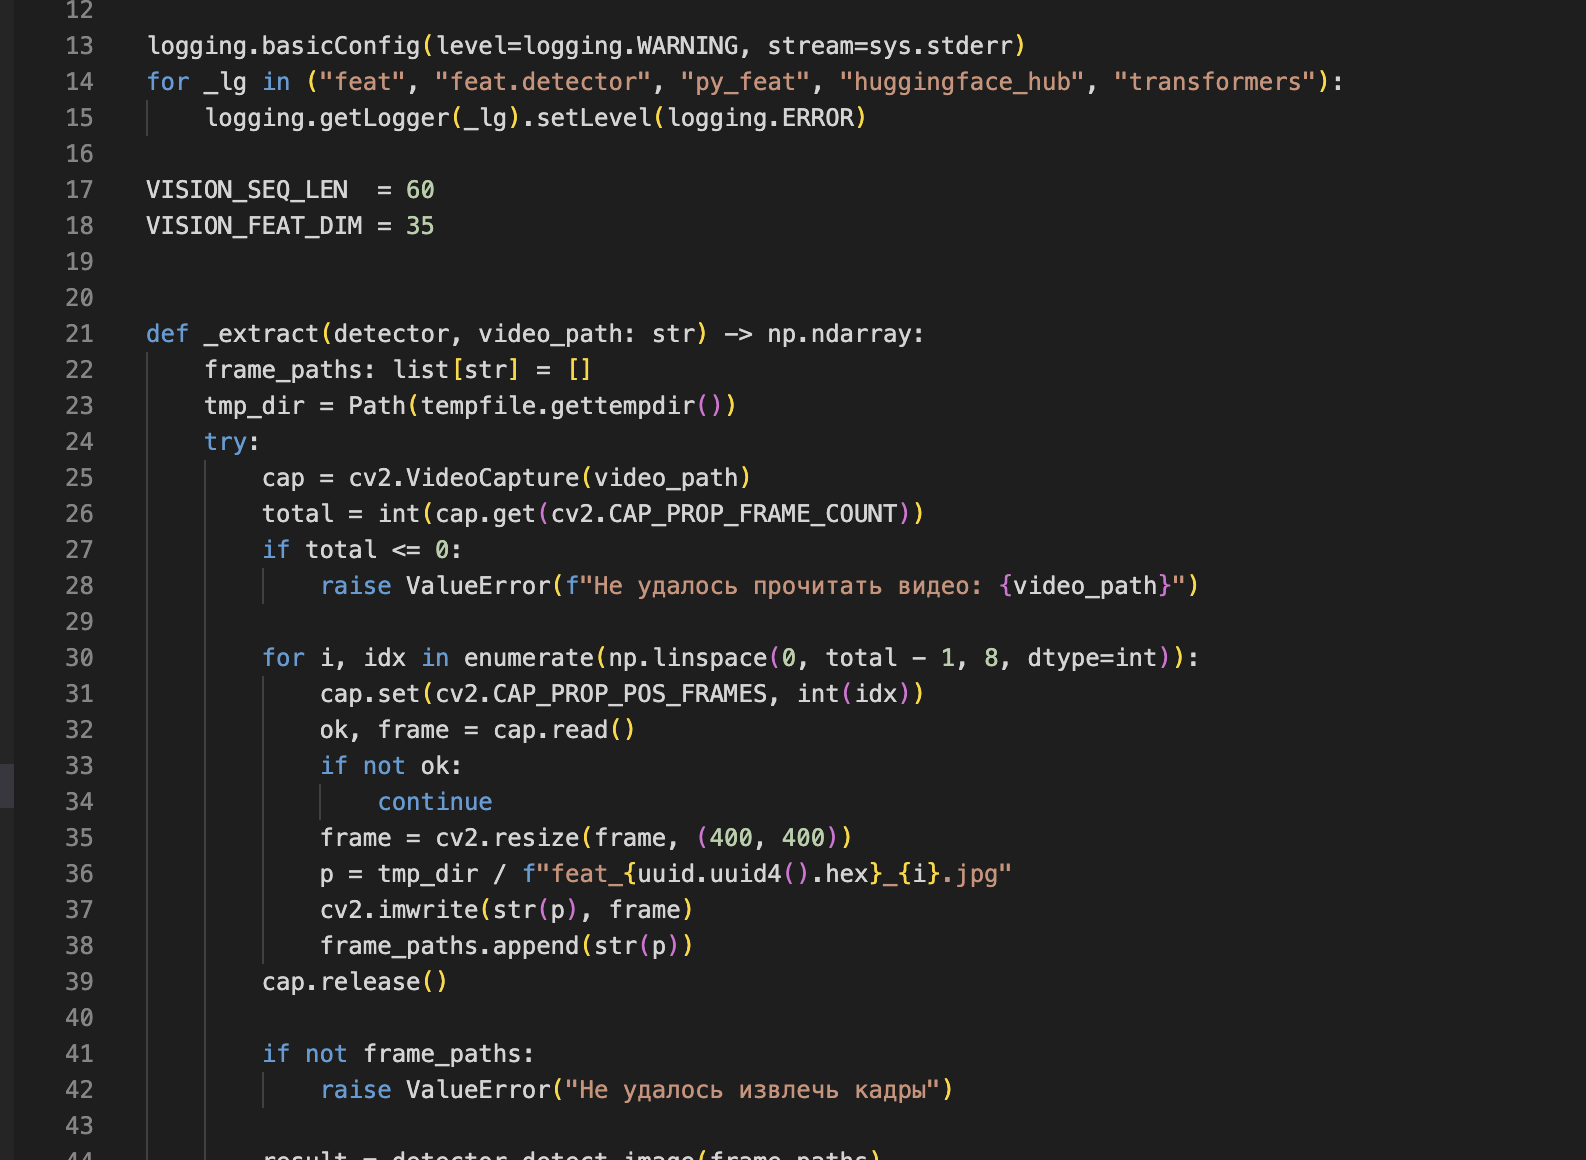
\includegraphics[width=1\textwidth]{images/videoextraxt.png}
    \caption{Video preprocessing and feature extraction pipeline}
    \label{fig:code_video}
\end{figure}


